\documentclass{lecture-kuznia}

\def\data{30.09.2026}
\def\place{Poręba Wielka}
\def\title{Kolorowanki i numerowanki}
\def\group{Juniorzy}
\def\author{Autor: Stefan Świerczewski}
\def\lecturer{Prowadzący: Stefan Świerczewski}

\begin{document}
\begin{center}
	{\LARGE\textbf{\title{}}}
\end{center}

\section{Teoria}

\subsection{Kredka jako wykrywacz oszustw}

W zadaniach kombinatorycznych kolorowanie rzadko służy do upiększania planszy.
Kolory mają pilnować, czego nie potrafi zmienić dozwolony ruch, klocek albo
operacja. Innymi słowy: kredka pracuje tu jako ochroniarz niezmiennika.

\begin{definition}
	Jeżeli pola planszy pomalowano na $k$ kolorów, to \emph{profilem kolorów}
	zbioru pól nazwiemy ciąg
	\[
		(c_1,c_2,\dots,c_k),
	\]
	gdzie $c_i$ oznacza liczbę pól w $i$-tym kolorze.
\end{definition}

Jeżeli każdy używany klocek ma profil $(1,1)$, to każda figura ułożona z tych
klocków musi mieć tyle samo pól obu kolorów. Jeśli plansza ma profil
$(30,32)$, możemy spokojnie odłożyć klej. Nie pomoże nawet bardzo stanowcze
dociskanie klocków.

\begin{example}\label{Edomino}
	Z szachownicy $8\times8$ usunięto dwa przeciwległe pola narożne. Czy
	pozostałą część można pokryć kostkami domina $1\times2$?
\end{example}

\begin{center}
	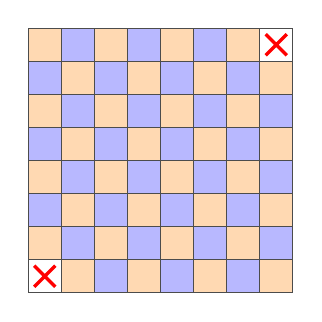
\begin{tikzpicture}[scale=0.42]
		\foreach \x in {0,...,7}{
			\foreach \y in {0,...,7}{
				\pgfmathtruncatemacro{\parity}{mod(\x+\y,2)}
				\ifnum\parity=0
					\fill[blue!28] (\x,\y) rectangle ++(1,1);
				\else
					\fill[orange!30] (\x,\y) rectangle ++(1,1);
				\fi
			}
		}
		\fill[white] (0,0) rectangle ++(1,1);
		\fill[white] (7,7) rectangle ++(1,1);
		\draw[red,very thick] (0.18,0.18)--(0.82,0.82) (0.82,0.18)--(0.18,0.82);
		\draw[red,very thick] (7.18,7.18)--(7.82,7.82) (7.82,7.18)--(7.18,7.82);
		\draw[step=1,black!70] (0,0) grid (8,8);
	\end{tikzpicture}
\end{center}

\begin{solution*}[\ref{Edomino}]
	Kolorujemy szachownicę jak zwykle. Każda kostka domina zakrywa jedno pole
	każdego koloru. Usunięte narożniki mają ten sam kolor, więc zostało
	$30$ pól tego koloru i $32$ pola drugiego. Domino domagałoby się równych
	liczb. Odpowiedź brzmi: nie.
\end{solution*}

\begin{remark}
	Kolorowanie dobieramy do klocka albo ruchu, nie do zasłon. Szachownica
	czarno-biała jest sławna, ale czasem potrzebujemy trzech, czterech albo
	więcej kolorów.
\end{remark}

\subsection{Więcej kredek, mniej możliwości}

Na prostokątnej planszy ponumerujmy wiersze i kolumny od zera. Pole $(i,j)$
możemy pokolorować kolorem odpowiadającym reszcie
	\[
		i+j\pmod k.
	\]
Każdy prosty klocek długości $k$, położony poziomo lub pionowo, przykrywa
wtedy po jednym polu każdego koloru.

Na planszy $10\times10$ cztery kolory dane przez $i+j\pmod4$ występują
w liczbach
	\[
		25,\quad 26,\quad 25,\quad 24.
	\]
Dlatego tej planszy nie da się pokryć prostokątami $1\times4$. Pole ma się
zgadzać, ale księgowość kolorów odmawia współpracy.

\subsection{Numerowanki, czyli kolory po kursie rachunkowości}

Kolor mówi tylko: „należę do tej grupy”. Numer potrafi powiedzieć więcej.
Każdemu polu albo obiektowi przypisujemy wagę, a potem obserwujemy sumę wag.

\begin{definition}
	Jeżeli na polu $P$ leży $n_P$ kamieni, a pole ma wagę $w(P)$, to
	\emph{sumą ważoną} układu nazwiemy
	\[
		W=\sum_P n_Pw(P).
	\]
\end{definition}

Jeżeli każdy dozwolony ruch zmienia $W$ o zero, to $W$ jest niezmiennikiem.
Jeżeli start i meta mają różne wartości $W$, do mety nie da się dojść. To
cała metoda. Najtrudniejsza część polega na wymyśleniu numerków, które mają
dobry zwyczaj nie zmieniać się podczas ruchu.

\begin{example}\label{Ezaby}
	Dwa żetony stoją na polach $0$ i $3$ nieskończonej taśmy. W jednym ruchu
	przesuwamy jeden żeton o jedno pole w lewo, a drugi o jedno pole w prawo.
	Czy żetony mogą kiedyś znaleźć się na tym samym polu?
\end{example}

\begin{solution*}[\ref{Ezaby}]
	Numer pola traktujemy jako jego wagę. Suma numerów żetonów wynosi na
	początku $3$. Każdy ruch zmniejsza jeden składnik o $1$ i zwiększa drugi
	o $1$, więc suma nadal wynosi $3$. Gdyby oba żetony spotkały się na polu
	$m$, suma wynosiłaby $2m$. Liczba $2m$ jest parzysta, a $3$ z uporem nie
	jest. Żetony mogą się minąć, ale na wspólną kawę nie trafią.
\end{solution*}

Kolorowanie jest szczególnym rodzajem numerowania. Zamiast zapisywać profil
$(c_1,\dots,c_k)$, możemy każdemu kolorowi przypisać osobną wagę albo
śledzić kilka sum jednocześnie. Czasem wygodniej myśleć kredkami, czasem
liczbami. Matematyka nie obraża się o zmianę narzędzia.

\subsection{Instrukcja obsługi}

Gdy widzimy planszę, klocki albo serię ruchów, warto sprawdzić:

\begin{enumerate}[itemsep=0pt,topsep=4pt]
	\item Jaki profil kolorów ma każdy klocek albo ruch?
	\item Czy reszty współrzędnych modulo $2$, $3$ albo $4$ tworzą wygodny wzór?
	\item Czy suma numerów, współrzędnych lub innych wag pozostaje stała?
	\item Czy start i meta mają ten sam profil albo tę samą sumę ważoną?
\end{enumerate}

Jeśli pierwsza próba nie działa, nie oznacza to, że zadanie jest odporne na
kredki. Być może wybraliśmy kredkę, która przyszła dziś tylko popatrzeć.

\newpage
\section{Zadania}

\begin{problem}[Rozgrzewka]\label{Z1}
	Z szachownicy $8\times8$ usunięto dwa pola. Udowodnij, że jeśli pozostałe
	pola można pokryć kostkami domina $1\times2$, to usunięte pola miały różne
	kolory w zwykłym kolorowaniu szachownicowym.
\end{problem}

\begin{problem}\label{Z2}
	Udowodnij, że planszy $10\times10$ nie można pokryć prostokątami
	$1\times4$ ułożonymi poziomo lub pionowo.
\end{problem}

\begin{problem}\label{Z3}
	Szachownicę $8\times8$ pokryto kostkami domina. Udowodnij, że liczba
	domin ułożonych poziomo jest parzysta.
\end{problem}

\begin{problem}[$\clubsuit$]\label{Z4}
	Z planszy $8\times8$ usunięto jedno pole, a pozostałe pola pokryto prostymi
	klockami $1\times3$, ułożonymi poziomo lub pionowo. Wiersze i kolumny
	ponumerowano od $1$ do $8$. Udowodnij, że usunięte pole $(i,j)$ spełnia
	\[
		i+j\equiv0\pmod3.
	\]
\end{problem}

\begin{problem}\label{Z5}
	Na zwykłej szachownicy $8\times8$ możemy w jednym ruchu zmienić kolor
	wszystkich pól w wybranym wierszu albo wybranej kolumnie. Czy można po
	pewnej liczbie ruchów otrzymać dokładnie $17$ białych pól?
\end{problem}

\begin{problem}[$\diamondsuit$]\label{Z6}
	Punkty prostokątnej kraty złożonej z $3$ wierszy i $7$ kolumn pomalowano
	na czerwono lub niebiesko. Udowodnij, że istnieje prostokąt o bokach
	równoległych do boków kraty, którego cztery wierzchołki mają ten sam kolor.
\end{problem}

% Motyw z wykładu kombinatorycznego dla juniorów, WM 2025.
\begin{problem}[$\diamondsuit$]\label{Z7}
	Jaś ponumerował wierzchołki sześcianu liczbami od $1$ do $8$, każdej
	używając dokładnie raz. Na każdej krawędzi napisał sumę liczb z jej
	końców. Udowodnij, że na dwóch krawędziach pojawiła się ta sama suma.
\end{problem}

% Motyw z wykładu kombinatorycznego dla juniorów, WM 2025.
\begin{problem}[$\redheart$]\label{Z8}
	W dwóch przeciwległych wierzchołkach jednej ściany sześcianu wpisano
	liczbę $1$, a w pozostałych wierzchołkach liczbę $0$. W jednym ruchu
	wybieramy krawędź i zwiększamy o $1$ liczby na obu jej końcach. Czy można
	doprowadzić do sytuacji, w której we wszystkich wierzchołkach stoi ta sama
	liczba?
\end{problem}

% 53. Olimpiada Matematyczna, etap I, zadanie 10; motyw obecny w WM 2025.
\begin{problem}[$\spadesuit$]\label{Z9}
	Na każdym polu szachownicy $2000\times2000$ leży jeden kamień. Jeśli na
	pierwszym i trzecim z trzech kolejnych pól jednego wiersza albo jednej
	kolumny leży kamień, możemy przełożyć oba te kamienie na pole środkowe.
	Czy można w ten sposób zebrać wszystkie kamienie na jednym polu?
\end{problem}

\begin{problem}[$\clubsuit$]\label{Z10}
	Czy skoczek szachowy może na planszy $5\times5$ odwiedzić każde pole
	dokładnie raz, a następnie jednym ruchem wrócić na pole, z którego
	wystartował?
\end{problem}

\begin{problem}[$\diamondsuit$]\label{Z11}
	W grupie jest $6$ osób. Dla każdej pary wiadomo, czy osoby z tej pary się
	znają. Udowodnij, że istnieją trzy osoby, które parami się znają, albo
	trzy osoby, z których żadne dwie się nie znają.
\end{problem}

% Motyw z wykładu kombinatorycznego dla juniorów, WM 2025.
\newpage
\begin{problem}[$\clubsuit$]\label{Z12}
	Na wyspie żyje $13$ zielonych, $15$ żółtych i $17$ czerwonych kameleonów.
	Gdy spotykają się dwa kameleony różnych kolorów, oba natychmiast przyjmują
	trzeci kolor. Czy może kiedyś dojść do sytuacji, w której:
	\begin{enumerate}[label= \alph*)]
		\item wszystkie kameleony mają ten sam kolor,
		\item każdego koloru jest tyle samo kameleonów?
	\end{enumerate}
\end{problem}

\begin{problem}[$\redheart$]\label{Z13}
	W wierzchołkach foremnego $2026$-kąta zapisano zera. W jednym ruchu
	wybieramy bok i zwiększamy o $1$ liczby na obu jego końcach. Czy można
	otrzymać układ, w którym w jednym wierzchołku stoi $1$, a we wszystkich
	pozostałych zera?
\end{problem}

\begin{problem}[$\spadesuit$]\label{Z14}
	Każdy punkt płaszczyzny o obu współrzędnych całkowitych pomalowano na jeden
	z $k$ kolorów. Udowodnij, że istnieje prostokąt o bokach równoległych do
	osi układu współrzędnych, którego cztery wierzchołki mają ten sam kolor.
\end{problem}

\begin{problem}[$\diamondsuit$]\label{Z15}
	Na wszystkich polach planszy $8\times8$ zapisano zera. W jednym ruchu
	wybieramy wiersz albo kolumnę i zwiększamy o $1$ wszystkie zapisane tam
	liczby. Czy można otrzymać układ, w którym liczby nieparzyste stoją
	dokładnie na głównej przekątnej planszy?
\end{problem}

\ifshowsolutions
\newpage
\section{Wskazówki}

\begin{hint*}[\ref{Z1}]
	Każde domino zużywa po jednym polu każdego koloru.
\end{hint*}

\begin{hint*}[\ref{Z2}]
	Pokoloruj pole $(i,j)$ według reszty $i+j$ z dzielenia przez $4$.
\end{hint*}

\begin{hint*}[\ref{Z3}]
	Pokoloruj całe kolumny na przemian na dwa kolory. Policz pola jednego
	koloru przykryte przez domina poziome.
\end{hint*}

\begin{hint*}[\ref{Z4}]
	Użyj trzech kolorów danych przez $i+j\pmod3$. Pełna plansza nie ma po
	równo pól wszystkich kolorów.
\end{hint*}

\begin{hint*}[\ref{Z5}]
	Sprawdź parzystość liczby białych pól po jednym ruchu.
\end{hint*}

\begin{hint*}[\ref{Z6}]
	W każdej kolumnie wybierz parę punktów tego samego koloru. Ile istnieje
	możliwych wyborów: para wierszy wraz z kolorem?
\end{hint*}

\begin{hint*}[\ref{Z7}]
	Załóż, że wszystkie $12$ sum są różne. Leżą one między $3$ i $15$.
	Policz ich łączną sumę, pamiętając, że każdy wierzchołek ma trzy krawędzie.
\end{hint*}

\begin{hint*}[\ref{Z8}]
	Pokoloruj wierzchołki sześcianu na dwa kolory tak, aby każda krawędź
	łączyła różne kolory. Śledź różnicę sum liczb w obu kolorach.
\end{hint*}

\begin{hint*}[\ref{Z9}]
	Każdemu polu przypisz numer wiersza i osobno numer kolumny. Co dzieje się
	z sumą numerów pól, na których leżą kamienie?
\end{hint*}

\begin{hint*}[\ref{Z10}]
	Skoczek po każdym ruchu zmienia kolor pola. Ile ruchów miałaby zamknięta
	trasa przez $25$ pól?
\end{hint*}

\begin{hint*}[\ref{Z11}]
	Wybierz jedną osobę. Spośród jej pięciu relacji co najmniej trzy są tego
	samego rodzaju.
\end{hint*}

\begin{hint*}[\ref{Z12}]
	Sprawdź modulo $3$ różnice między liczbami kameleonów poszczególnych
	kolorów.
\end{hint*}

\begin{hint*}[\ref{Z13}]
	Wierzchołkom przypisz na przemian wagi $1$ i $-1$.
\end{hint*}

\begin{hint*}[\ref{Z14}]
	Spójrz na $k+1$ ustalonych kolumn kraty. Możliwych wzorów kolorów w jednym
	wierszu jest skończenie wiele.
\end{hint*}

\begin{hint*}[\ref{Z15}]
	Obserwuj parzystość sumy liczb w prostokącie utworzonym przez wiersze
	$1,2$ i kolumny $2,3$.
\end{hint*}

\newpage
\section{Rozwiązania}

\begin{solution*}[\ref{Z1}]
	W zwykłym kolorowaniu każde domino przykrywa jedno pole białe i jedno
	czarne. Cała szachownica ma po $32$ pola obu kolorów. Po usunięciu dwóch
	pól pozostałe liczby muszą być równe, więc usunęliśmy po jednym polu
	każdego koloru.
\end{solution*}

\begin{solution*}[\ref{Z2}]
	Numerujemy wiersze i kolumny od $0$ do $9$ i kolorujemy pole $(i,j)$
	według reszty $i+j$ modulo $4$. Każdy klocek $1\times4$, niezależnie od
	ułożenia, przykrywa po jednym polu każdego koloru.

	W dziesięciu kolejnych polach jednego wiersza kolory występują w liczbach
	$3,3,2,2$, w kolejnych wierszach wzór przesuwa się cyklicznie. Po zliczeniu
	całej planszy otrzymujemy liczności $25,26,25,24$. Nie są równe, więc
	pokrycie nie istnieje.
\end{solution*}

\begin{solution*}[\ref{Z3}]
	Kolumny kolorujemy na przemian na biało i czarno. Mamy $32$ czarne pola.
	Niech $h$ oznacza liczbę domin poziomych. Każde z nich przykrywa dokładnie
	jedno czarne pole. Domino pionowe przykrywa albo dwa czarne pola, albo
	żadnego. Zatem
	\[
		32=h+2v
	\]
	dla pewnej liczby całkowitej $v$. Stąd $h$ jest parzyste.
\end{solution*}

\begin{solution*}[\ref{Z4}]
	Pole $(i,j)$ kolorujemy według reszty $i+j$ modulo $3$. Każdy klocek
	$1\times3$ przykrywa po jednym polu każdego koloru.

	Na pełnej planszy $8\times8$ kolory występują w liczbach $22,21,21$.
	Dokładnie $22$ razy występuje kolor odpowiadający reszcie $0$, czyli pola
	z $i+j\equiv0\pmod3$. Po usunięciu jednego pola i ułożeniu $21$ klocków
	każdy kolor musi wystąpić dokładnie $21$ razy. Usunięto więc pole koloru
	$0$.
\end{solution*}

\begin{solution*}[\ref{Z5}]
	Na początku są $32$ białe pola. Jeżeli w wybranym wierszu albo kolumnie
	jest $b$ białych pól, po ruchu będzie ich tam $8-b$. Łączna liczba białych
	pól zmieni się o
	\[
		(8-b)-b=8-2b,
	\]
	czyli o liczbę parzystą. Jej parzystość zawsze pozostaje więc parzysta.
	Liczby $17$ otrzymać nie można.
\end{solution*}

\begin{solution*}[\ref{Z6}]
	W każdej kolumnie spośród trzech punktów co najmniej dwa mają ten sam
	kolor. Dla tej kolumny wybieramy jedną taką parę i zapisujemy: które dwa
	wiersze wybraliśmy oraz jaki jest ich wspólny kolor.

	Są trzy pary wierszy i dwa kolory, a więc tylko $6$ możliwych zapisów.
	Kolumn jest $7$. Z zasady szufladkowej dwie kolumny otrzymały ten sam
	zapis. W odpowiedniej parze wierszy i tych dwóch kolumnach leżą cztery
	wierzchołki prostokąta jednego koloru.
\end{solution*}

\begin{solution*}[\ref{Z7}]
	Załóżmy przeciwnie, że wszystkie sumy na $12$ krawędziach są różne.
	Każda z nich leży między $1+2=3$ i $7+8=15$. W przedziale od $3$ do $15$
	jest $13$ liczb, więc na krawędziach stoją wszystkie z wyjątkiem jednej,
	powiedzmy $k$.

	Każda liczba z wierzchołka pojawia się w sumach na trzech krawędziach,
	więc suma wszystkich napisów na krawędziach wynosi
	\[
		3(1+2+\cdots+8)=108.
	\]
	Z drugiej strony
	\[
		3+4+\cdots+15=117,
	\]
	zatem $117-k=108$ i $k=9$. W szczególności występują sumy $3,4,5,6$.

	Suma $3$ wymusza krawędź $1$--$2$, a suma $4$ krawędź $1$--$3$.
	W sześcianie dwaj różni sąsiedzi jednego wierzchołka nie są połączeni,
	więc $2$ i $3$ nie sąsiadują. Suma $5$ musi zatem pochodzić z krawędzi
	$1$--$4$. Wierzchołek $1$ ma już wszystkich trzech sąsiadów: $2,3,4$.
	Suma $6$ mogłaby pochodzić tylko z krawędzi $1$--$5$ albo $2$--$4$.
	Pierwsza nie istnieje, bo $1$ ma stopień $3$, a druga nie istnieje, bo
	$2$ i $4$ są różnymi sąsiadami wierzchołka $1$. Sprzeczność.
\end{solution*}

\begin{solution*}[\ref{Z8}]
	Kolorujemy wierzchołki sześcianu na czarno i biało tak, aby końce każdej
	krawędzi miały różne kolory. Każda klasa ma po cztery wierzchołki.
	Przeciwległe wierzchołki jednej ściany mają ten sam kolor, więc na początku
	różnica sum liczb w obu klasach wynosi $2$ albo $-2$.

	W każdym ruchu zwiększamy o $1$ jedną liczbę w każdym kolorze. Różnica sum
	pozostaje zatem stała. Gdyby wszystkie liczby stały się równe $t$, obie
	sumy wynosiłyby $4t$, a ich różnica byłaby równa zero. To niemożliwe.
\end{solution*}

\begin{solution*}[\ref{Z9}]
	Każdemu kamieniowi przypisujemy jako wagę numer wiersza pola, na którym
	leży. Ruch poziomy nie zmienia żadnej z tych wag. W ruchu pionowym dwa
	kamienie z wierszy $r-1$ i $r+1$ trafiają do wiersza $r$, więc ich łączna
	waga zmienia się z
	\[
		(r-1)+(r+1)=2r
	\]
	na $r+r=2r$. Suma numerów wierszy wszystkich kamieni jest niezmienna.

	Początkowo średni numer wiersza kamienia wynosi
	\[
		\frac{1+2000}{2}=1000{,}5.
	\]
	Gdyby wszystkie kamienie znalazły się na jednym polu, ich średni numer
	wiersza byłby całkowity. Otrzymujemy sprzeczność. Nie da się zebrać
	wszystkich kamieni na jednym polu. Tak samo można śledzić numery kolumn,
	ale jeden niezmiennik w zupełności wystarcza do zatrzymania tej przeprowadzki.
\end{solution*}

\begin{solution*}[\ref{Z10}]
	Kolorujemy planszę jak szachownicę. Każdy ruch skoczka zmienia kolor pola,
	bo jedna współrzędna zmienia się o $1$, a druga o $2$.

	Zamknięta trasa odwiedzająca każde z $25$ pól dokładnie raz miałaby
	$25$ ruchów: po jednym między kolejnymi polami i ostatni z powrotem do
	początku. Po nieparzystej liczbie ruchów skoczek znajduje się na polu
	innego koloru niż początkowe, więc nie może do niego wrócić. Taka trasa
	nie istnieje.
\end{solution*}

\begin{solution*}[\ref{Z11}]
	Wybieramy osobę $A$. Spośród pozostałych pięciu osób co najmniej trzy
	albo znają $A$, albo jej nie znają.

	Załóżmy najpierw, że $A$ zna osoby $B,C,D$. Jeżeli jakaś para spośród
	$B,C,D$ się zna, to wraz z $A$ tworzy trójkę parami znajomych. Jeżeli
	żadna taka para się nie zna, osoby $B,C,D$ tworzą trójkę parami
	nieznajomych.

	Jeżeli natomiast $A$ nie zna trzech osób $B,C,D$, rozumowanie jest
	analogiczne: para nieznajomych wśród nich wraz z $A$ daje trójkę
	nieznajomych, a jeśli każda para się zna, mamy trójkę znajomych.
\end{solution*}

\begin{solution*}[\ref{Z12}]
	Oznaczmy liczby zielonych, żółtych i czerwonych kameleonów przez $z,y,c$.
	Spotkanie dwóch różnych kolorów zmienia te liczby, w pewnej kolejności,
	tak:
	\[
		(z,y,c)\longmapsto(z-1,y-1,c+2).
	\]
	Modulo $3$ wszystkie trzy liczby zmniejszają się więc o $1$. Wobec tego
	różnice $z-y$, $y-c$ i $c-z$ modulo $3$ pozostają stałe.

	Na początku liczby $13,15,17$ dają trzy różne reszty $1,0,2$ modulo $3$.
	Zarówno w układzie jednokolorowym $(45,0,0)$, jak i w układzie
	$(15,15,15)$ wszystkie trzy liczby mają tę samą resztę modulo $3$.
	Żadna z opisanych sytuacji nie może zatem wystąpić.
\end{solution*}

\begin{solution*}[\ref{Z13}]
	Wierzchołkom wielokąta przypisujemy na przemian wagi $1$ i $-1$. Jest to
	możliwe, bo liczba wierzchołków jest parzysta. Śledzimy sumę liczb
	zapisanych w wierzchołkach, pomnożonych przez odpowiadające im wagi.

	Końce każdego boku mają przeciwne wagi. Ruch zwiększa więc sumę ważoną o
	$1-1=0$. Na początku suma wynosi zero. Układ z jedną jedynką i pozostałymi
	zerami ma sumę ważoną równą $1$ albo $-1$, więc nie można go otrzymać.
\end{solution*}

\begin{solution*}[\ref{Z14}]
	Ustalamy $k+1$ pionowych prostych kraty, na przykład o współrzędnych
	$x=0,1,\dots,k$. Każdy poziomy wiersz wyznacza na tych prostych ciąg
	$k+1$ kolorów. Takich ciągów jest tylko $k^{k+1}$, a wierszy mamy
	nieskończenie wiele. Dwa różne wiersze mają zatem dokładnie ten sam ciąg
	kolorów.

	W jednym z tych wierszy leży $k+1$ punktów pomalowanych na $k$ kolorów.
	Dwa z nich mają ten sam kolor. Punkty w tych samych dwóch kolumnach
	i w drugim wybranym wierszu mają identyczne kolory. Otrzymaliśmy cztery
	jednokolorowe wierzchołki prostokąta.
\end{solution*}

\begin{solution*}[\ref{Z15}]
	Rozważamy cztery pola leżące w wierszach $1,2$ i kolumnach $2,3$.
	Początkowo suma zapisanych w nich liczb jest parzysta. Każdy ruch zmienia
	albo zero, albo dwie liczby w tym prostokącie, więc parzystość ich sumy
	pozostaje stała.

	W żądanym układzie spośród tych czterech pól tylko pole $(2,2)$ leży na
	głównej przekątnej. Stałaby na nim liczba nieparzysta, a na pozostałych
	trzech liczby parzyste. Ich suma byłaby nieparzysta, co przeczy
	niezmiennikowi. Takiego układu nie można otrzymać.
\end{solution*}
\fi

\end{document}
